\chapter{システムの実装方法}
\label{chp:reference}

\section{システム構成}
\label{sec:reference_ftnote}
本システムは以下のような構成で実装を行う.システム構成図を図3.1に示す.\\
労務管理支援システムをReactでWebアプリとして作成した.さらにデータベースにCloud Firestore,
ユーザー認証にFirebase Authentication,表情分析にface-api.jsを使用した。\\
 次のセクションでは,それぞれのサービスについて説明する.

\begin{figure}[!h]
	\begin{center}
			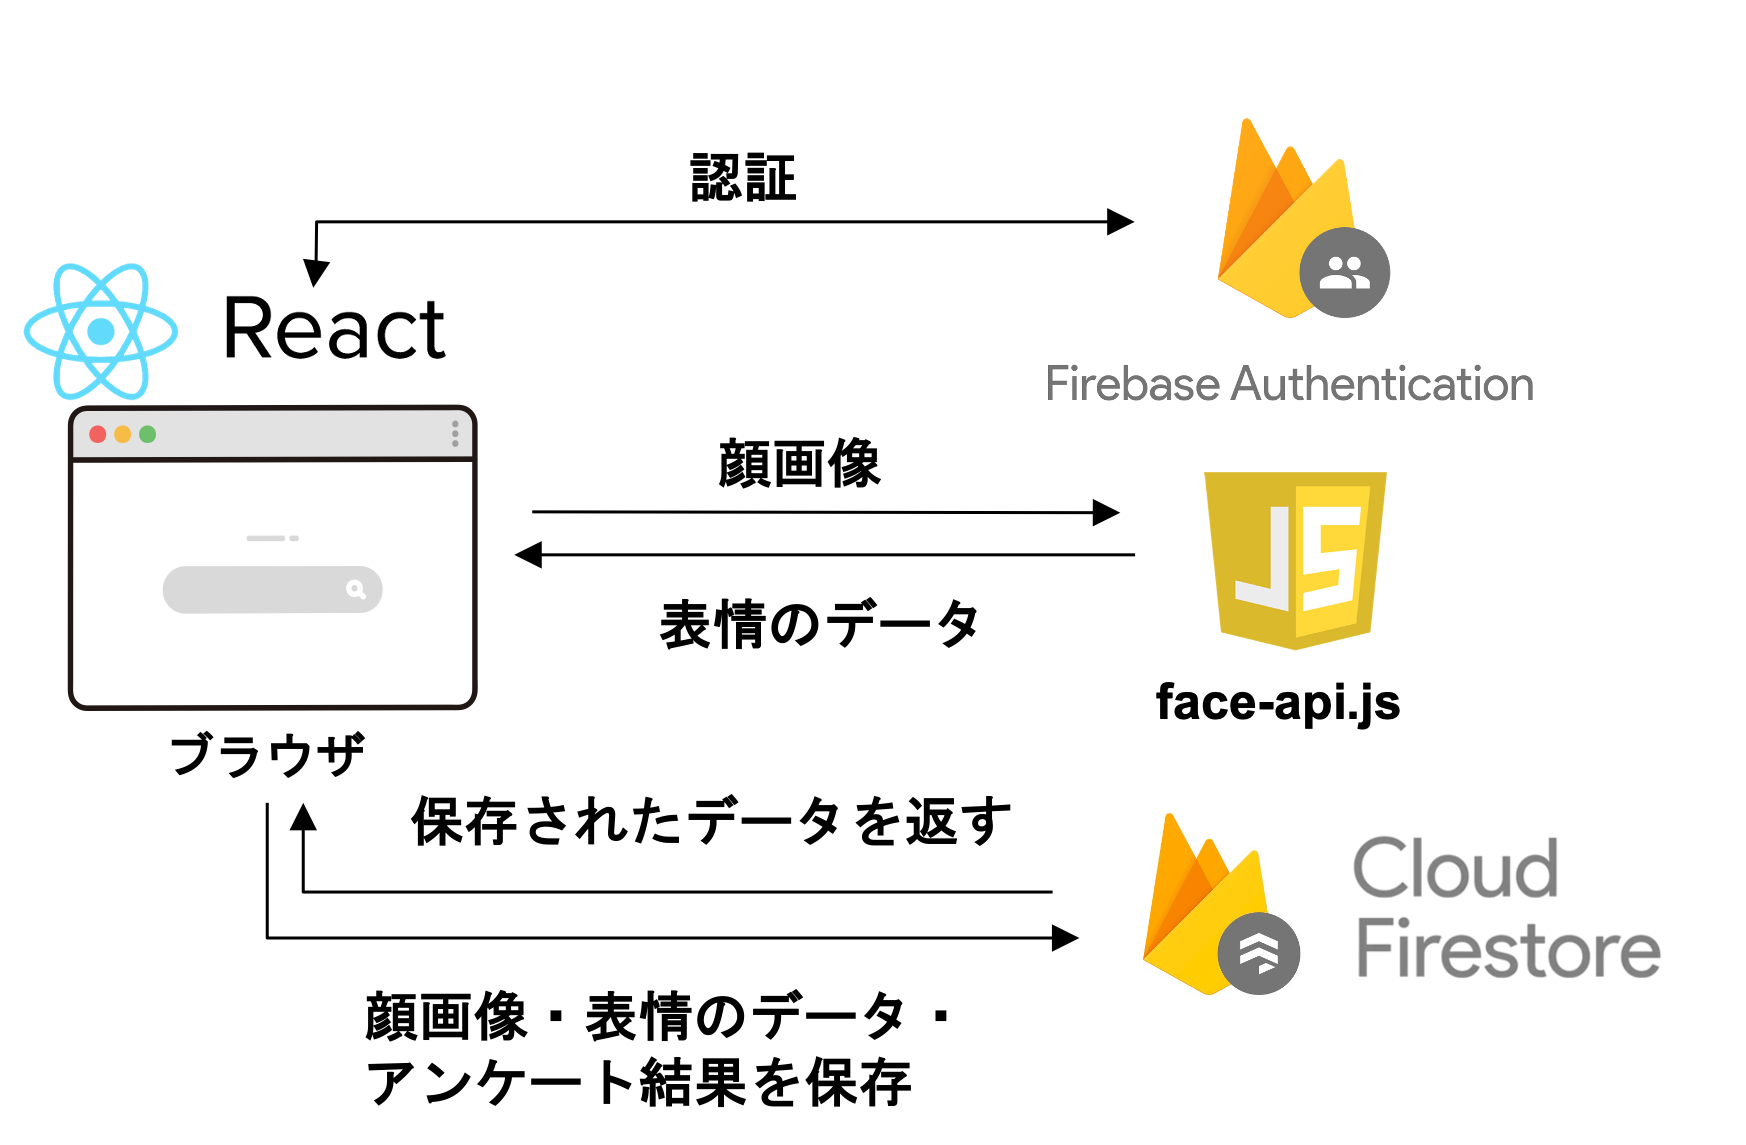
\includegraphics[scale=1.2, clip]{./img/compose.png}
			\caption{システム構成図}
			\label{fig:図の名前}
	\end{center}
\end{figure}


\section{React}
\label{sec:reference_quote}
	Reactとは, Facebook社が開発したWebサイト上のUIパーツを構築するためのJavaScriptライブラリである.
	今回のシステム開発にReactを採用した理由は三つある.

	\begin{enumerate}
		\item パフォーマンスが良い \\
		Reactには,仮想DOM(Virtual Document Object Model)というレンダリング機構が
		備わっている.仮装DOMとは、実際のDOMではなく, React内部に持っている 
		DOMの情報である. Reactを使うと,この仮想DOMと実際のHTML上のDOMを
		比較したときに出てくる違いだけが,毎回HTML上に再適用される.
		そのため画面全体がReactで構成されていたとしても,必要な部分しか更新されず
		非常に高速に動作するため,パフォーマンスが良い.\\
		\item UIコンポーネントのライブラリが多い \\
		Reactは、世界中で使われているため、Reactのライブラリを使ってUIをコンポート化
		するようになってきています。あらかじめButton や Form などの UI パーツを
		React コンポーネントとして扱えるようにして、セット化したものが多くあります。
		これらを使えば、今風の洗練された画面を作ることができるでしょう。\\
		\item JavaScriptの知識があれば使える \\
	\end{enumerate}
	

\section{face-api.jsについて}
\label{sec:reference_bib}
	

\section{Material-UIについて}
\label{sec:reference_chapter}
	